\chapter{Umsetzung von Kommunikationsschemen über Kafka}
\newcommand{\C}{\textit{Consumer}}
\newcommand{\Cn}{\textit{Consumern}}
\newcommand{\CG}{\textit{Consumer Group}}
\newcommand{\CGs}{\textit{Consumer Groups}}
\newcommand{\T}{\textit{Topic}}
\newcommand{\Tcs}{\textit{Topics}}
\newcommand{\Pt}{\textit{Partition}}
\newcommand{\Pts}{\textit{Partitionen}}
\newcommand{\Pd}{\textit{Producer}}
\newcommand{\Evs}{\textit{Events}}
\newcommand{\Ev}{\textit{Event}}
Um Hamaube skalierbar aufsetzen zu können, musste auf die Skalierbarkeit der Kommunikation zwischen den Komponenten geachtet werden. In diesem Kapitel wird beschrieben, welche Techniken eingesetzt wurden, um die Skalierbarkeit der Kommunikation zu gewährleisten. Hierfür werden zunächst die benötigten Grundlagen bezüglich Kafka beschrieben und anschließend wird auf die Realisierung von zwei Kommunikationsschemen mithilfe von Kafka eingegangen.
\section{Grundlagen Kafka}
\subsection{Registrieren eines Consumers}
Wird eine Nachricht über eine Kafka-Instanz verbreitet, so ist sie einem \T\ zugeordnet.
Möchte eine Komponente von Kafka Nachrichten erhalten, muss sie sich als \C\ regieren. Hierbei muss sie mindestens ein \T\ angeben, an dem sie interessiert ist, sowie eine \CG. Wird nun eine Nachricht über Kafka verbreitet, wird ein \C\ jeder \CG, der an dem \T der Nachricht interessiert ist, ausgewählt und die Nachricht diesen \C\ weitergeleitet. Abbildung \ref{fig:exampleKafkaConsumerRegistration} zeigt ein Beispiel für die Zuordnung von \Cn\ zu \CGs\ und die Registrierung der \C\ bei \Tcs. Wird in diesem Beispiel ein Nachricht für \T\ 2 hinterlegt, so werden \C\ 1 oder \C\ 2, sowie \C\ 4 informiert. Wird allerdings eine Nachricht für \T\ 1 hinterlegt, wird nur \C\ 1 oder \C\ 2 informiert.
\begin{figure}
	\caption{Beispiel für die Zuordnung von \Cn\ zu \CGs\ und \Tcs.}
	\label{fig:exampleKafkaConsumerRegistration}
	\centering
	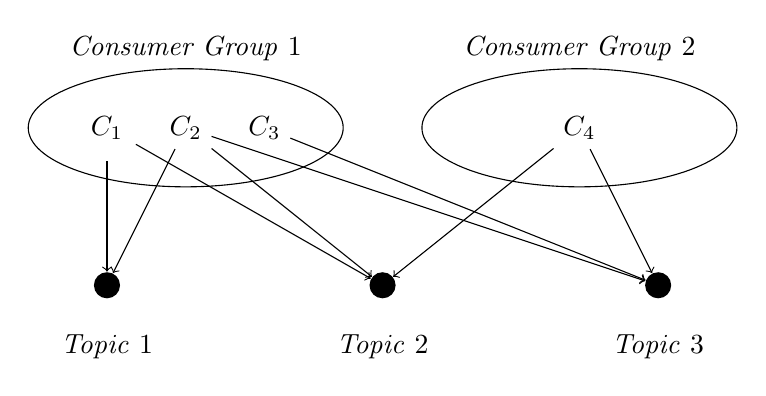
\begin{tikzpicture}
		\draw (0,0) ellipse (2cm and 0.75cm);
		\node (CG2) at (0,1) {\CG\ 1};
		\draw (5,0) ellipse (2cm and 0.75cm);
		\node (CG2) at (5,1) {\CG\ 2};
		\node[fill=black, circle] (T1) at (-1,-2) {};
		\node[fill=black, circle] (T2) at (2.5,-2) {};
		\node[fill=black, circle] (T3) at (6,-2) {};
		\node[below=0.5cm] at (T1) {\T\ 1};
		\node[below=0.5cm] at (T2) {\T\ 2};
		\node[below=0.5cm] at (T3) {\T\ 3};
		\node[circle, minimum size=0.1cm] (C1) at (-1,0) {$C_1$};
		\node (C2) at (0,0) {$C_2$};
		\node (C3) at (1,0) {$C_3$};
		\node (C4) at (5,0) {$C_4$};
		\path[->] (C1) edge (T1) edge (T2)
		(C2) edge (T1) edge (T2) edge (T3)
		(C3) edge (T3)
		(C4) edge (T2) edge (T3);
	\end{tikzpicture}
\end{figure}
\subsection{Nachrichtenverteilung}
Haben sich mehrere \C\ einer \CG\ bei Kafka registriert, um Nachrichten für ein \T\ zu erhalten, werden diesen \Cn\ zunächst \Pts\ zugeordnet. Erhält Kafka nun eine Nachricht für ein \T, kann entweder vom \Td\ - also dem Sender der Nachricht - festgelegt werden, in welche Partition die Nachricht gelegt werden soll, oder Kafka teilt die Nachricht so einer Partition zu, dass die Nachrichten möglichst gleichverteilt den \Tcs\ zugeordnet werden. Nachdem die Nachricht einer \Pt\ zugeordnet ist, wird sie dem \C\ einer jeden \CG\ übermittelt, dem die \Pt\ zugeteilt ist. \\
Für die Zuordnung der \Pts\ zu den \Cn\ einer jeden \CG\ wird eine Zuordnungsstrategie verwendet. Hier liefert Kafka die beiden Strategien \glqq range\grqq\ und \glqq roundrobin\grqq\ mit, von denen eine ausgewählt werden kann. Alternativ lässt sich eine eigene Zuordnungsstrategie definieren.
\section{Realisierung der Kommunikationsschemen}
In unserem Projekt \glqq Hamaube\grqq\ haben wir die Semantik der Nachrichten so gewählt, dass sie als \Evs\ zu verstehen sind. Diese \Evs\ können potentiell von einer beliebigen Instanz ausgelesen werden. So ist beispielsweise unsere Analyseinstanz an mehrere \Tcs\ angeschlossen, um Analysen über die Nutzung von Hamaube bzw. die Twitterdaten durchzuführen. \\
\\
Trotz dieser \Ev-Charakteristik haben viele Nachrichten ein primäres Ziel. So hat beispielsweise ein \Ev\, das signalisiert, dass sich ein Anwender einen Webserver nach seine Timeline gefragt hat, das primäre Ziel, dass es von einem beliebigen Datenbank-Server aufgenommen wird, um die Einträge der Timeline aus der Datenbank zu laden. Anschließend sollte diese Datenbank-Server ein \Ev\ verschicken, das signalisiert, welche Einträge dem Anwender angezeigt werden sollen. Dieses \Ev\ hat wiederum das primäre Ziel, dass der entsprechende Webserver die Anfrage des Nutzers beantworten kann. Im Folgenden wird die Komponente, die das \Ev\ primär erhalten soll, Kommunikationspartner genannt.
\subsection{Beliebiger Kommunikationspartner}
Für viele Nachrichten, die Hamaube über Kafka verschickt, reicht es, wenn eine beliebige Instanz einer bestimmten Gruppe von Servern das Event erhält. Wenn beispielsweise ein Webserver einen Datenbank-Server darüber informieren möchte, dass die Einträge einer Timeline geladen werden sollten, ist für den Webserver egal, welcher Datenbank-Server das Event zur Bearbeitung der Anfrage erhält.\\
Soll ein beliebiger Kommunikationspartner für ein Event ausgewählt werden, kann das Event von Kafka einer beliebigen Partition zugeteilt werden und eine der beiden Standard Zuordnungsstrategien gewählt werden, um die Partitionen den \Cn\ der \CG\ zuzuordnen.
\subsection{Ausgewählter Kommunikationspartner}
In einigen Fällen, ist das \Ev\ allerdings primär nur für eine Instanz entscheidend. So sollte das \Ev, dass die Einträge einer Timeline enthält beispielsweise möglichst direkt den Webserver erreichen, an dem die Timeline angefragt wurde. Um dies zu realisieren, könnte der Webserver der Anfrage seine ID mitschicken und dann das Antwort-\T\ nach seiner ID filtern. Diese Lösung würde allerdings dazu führen, dass die Kommunikation nicht mehr skalierbar wäre, da dann jeder Webserver jede Antwort auf jede Anfrage erhalten müsste und zum Filter der Antworten bearbeiten müsste. Dies ließe sich nicht skalierbar realisieren. Die \C\ müssen also der selben \CG\ zugeordnet sein. \\
Um nun zu gewährleisten, dass der Webserver, der die Anfrage gestellt hat, die Antwort erhält, muss die Antwort zum einen in eine feste \Pt\ gelegt werden und zum anderen musste eine Strategie für die Zuordnung von Partitionen auf die \C\ implementiert werden, mit der garantiert werden kann, dass die Antwort auch bei erneuter Verteilung der \Pts\ beim richtigen \C\ landet. Dies können beide von Kafka mitgelieferten Verteilungsstrategien nicht gewährleisten, wie in Abbildung \ref{fig:roundrobin} beispielhaft für das \glqq roundrobin\grqq-Verfahren dargestellt.
\begin{figure}
	\caption{Beispiel für die Umverteilung der Partitionen mit dem \glqq roundrobin\grqq\ Verfahren: Zwischen Zustand 1 und Zustand 2 wurde der Consumer 2 entfernt.}
	\label{fig:roundrobin}	
	\centering
	\textbf{Zustand 1:} \\
	\begin{tabular}{c | c | c}
		Consumer 1 & Consumer 2 & Consumer 3 \\
		\hline
		Partition 1 & Partition 2 & Partition 3 \\
		Partition 4 & Partition 5
	\end{tabular} \\[0.5cm]
	\textbf{Zustand 2:} \\
	\begin{tabular}{c | c}
	Consumer 1 & Consumer 3 \\
	\hline
	Partition 1 & Partition 2 \\
	Partition 3 & Partition 4 \\
	Partition 5
	\end{tabular}
\end{figure} \\
\\
Wird eine Webserver-Instanz von Hamaube gestartet, muss ihr eine Partitionsnummer als Argument übergeben werden. Registriert sich die Webserver-Instanz bei Kafka als Consumer, kann sie eine ID übergeben, die später an den Verteilungsalgorithmus für die Partitionen weitergegeben wird. Durch die ID kann der selbst implementierte Verteilungsalgorithmus erkennen welche Partition diesem Consumer zugeordnet werden muss. Ist eine Partition vorhanden, für die kein Consumer existiert, dessen ID die Nummer der Partition enthält, wird die Partition einem beliebigen Consumer zugeordnet.\\
\\
Schickt ein Webserver nun eine Anfrage an einen Datenbank-Server, enthält diese Anfrage ein Feld, das die Partition angibt, in die die Antwort gelegt werden soll. Durch den Verteilungsalgorithmus für die Partitionen ist garantiert, dass dem Webserver, solange er erreichbar ist, diese Partition zugeordnet ist, sodass nur er die Antwort erhält. Ist der Webserver nicht mehr erreichbar, wird seine Partition einem anderen Webserver zugeordnet, der die Antwort erhält und verwirft, da er sie Anfrage nicht gestellt hat. Die Antwort ist in diesem Falle also verloren.
